\chapter{Programmazione aggregata}\label{ch:aggregate}

\unsure[inline]{
  Alcuni concetti di programmazione aggregata, come le dicevo per mail, mi hanno richiesto un po' di tempo per saperli spiegare.

  Spero di non aver capito male delle cose o essere stato impreciso.
}

La crescita esponenziale di dispositivi informatici di varia natura inseriti in contesti quotidiani ha avuto un impatto globale notevole.
Questo insieme di entità connesse (\Cref{fig:iot}) ha dato luogo a ciò che viene definito \emph{Internet of Things} (\emph{IoT}).

\begin{figure}[htbp]
  \centering
  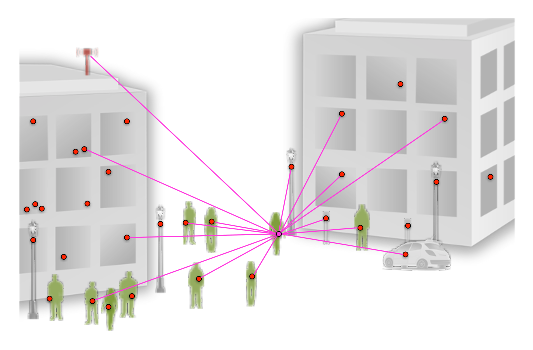
\includegraphics[width=0.8\textwidth]{res/fig/iot.eps}%
  \caption[
    Possibile scenario di rete in contesto urbano.
  ]{
    Possibile scenario di rete in contesto urbano.

    \nameCref{fig:iot} ripresa da~\cite{7274429}.
  }%
  \label{fig:iot}
\end{figure}

L'approccio tradizionale per la realizzazione di sistemi in questo contesto è sempre stato con paradigma ``\emph{single device view point}'',
in cui l'unità fondamentale è il singolo dispositivo connesso con il mondo fisico e con gli altri device, il cui insieme dei comportamenti individuali determinava il funzionamento del sistema.
Tale approccio si è rivelato inadeguato, in quanto un elevato numero di dispositivi (possibilmente eterogenei) pone diversi problemi legati all'organizzazione della rete
e la sua gestione che non dovrebbero essere gestiti in questo livello di astrazione.

L'\emph{aggregate programming}, o \emph{programmazione aggregata}, costituisce un'alternativa all'approccio ``classico''
volta a semplificare la progettazione, creazione e manutenzione di sistemi distribuiti complessi.
La programmazione aggregata, infatti, ragiona su più larga scala, cercando di spostare l'attenzione sul \emph{collettivo di dispositivi} che collaborano;
i dettagli relativi al singolo device devono essere ignorabili, per quanto possibile~\cite{7274429}.

L'idea alla base è dunque di definire una modalità di deduzione del comportamento locale al singolo dispositivo a partire dal comportamento globale, di più alto livello,
effettuando un \emph{mapping da globale a locale}.
I due punti di vista necessari per poter raggiungere un tale livello di astrazione sono due~\cite{aggregatescala-pmldc2016}:

\begin{itemize}
    \item
        il primo, detto locale o \emph{device-centric}, è quello che si riferisce alla computazione aggregata eseguita dal dispositivo singolo.
        Questa può essere considerata la vista tradizionale.
    \item
        il secondo, detto globale o \emph{aggregate view}, si riferisce invece alla computazione svolta dal sistema aggregato come singola unità.
        Rispetto all'approccio tradizionale, tale punto di vista sposta maggiormente l'attenzione dal \emph{come} il sistema possa funzionare
        al \emph{cosa} effettivamente si desidera che faccia.
\end{itemize}

In generale, le strategie principali per adottare un livello di astrazione così elevato sono state formalizzate nelle seguenti possibilità~\cite{7274429}:

% TODO: rielabora traduzione
\begin{itemize}
  \item rendere le interazioni tra i dispositivi implicite (come ad esempio nell'approccio \emph{TOTA}, ``\emph{Tuples On The Air}''~\cite{10.1145/1538942.1538945});
  \item comporre comporre costruzioni geometriche e topologiche (ad esempio, \emph{Origami Shape Language}~\cite{nagpal2001programmable});
  \item dividere la computazione in modo automatico per le esecuzioni sullo stile di modelli di \emph{computazione cloud} come \emph{MapReduce}~\cite{10.1145/1327452.1327492};
  \item sintetizzare i dati provenienti da regioni spazio-temporali e inviarli come stream ad altre regioni (ad esempio, \emph{TinyDB}~\cite{1017485});
  \item fornire costrutti generalizzabili per la computazione spazio-temporale (ad esempio, \emph{Protelis}~\cite{PianiniSASOTutorial2017}, di cui tratteremo meglio in~\Cref{sec:protelis}).
\end{itemize}

Studiando i suddetti approcci, sono state osservate le seguenti proprietà dei sistemi situati su larga scala:

% TODO: rielabora traduzione
\begin{itemize}
  \item laddove non è richiesta al programmatore alcuna interazione, i meccanismi per la coordinazione devono essere nascosti ``\emph{under the hood}''~\cite{7274429};
  \item la composizione dei moduli deve essere tanto semplice quanto trasparente;
  \item sottoinsiemi differenti necessitano di meccanismi di coordinazione differenti per regioni e tempi distinti.
\end{itemize}

Per affrontare queste problematiche, la programmazione aggregata si basa sui seguenti tre principi~\cite{7274429}:

\begin{itemize}
  \item la ``macchina'' programmata non deve essere il singolo dispositivo, bensì la \emph{regione} dell'ambiente computazionale che astrae dai dettagli specifici;
  \item il ``programma'' è specificato come \emph{manipolazione di costrutti di dati} con estensioni spaziali e temporali in tutta la regione;
  \item tali manipolazioni vengono eseguite dai dispositivi inseriti all'interno della regione, tramite l'uso di meccanismi di coordinazione resilienti e di interazioni basate sulla prossimità.
\end{itemize}

In questo modo, i meccanismi di coordinazione, spesso complessi, vengono nascosti facilitando la costruzione e favorendo la modularità.
In particolare, il paradigma si struttura su più livelli di astrazione, come è possibile vedere in~\Cref{fig:stack}.

\begin{figure}[htbp]
  \centering
  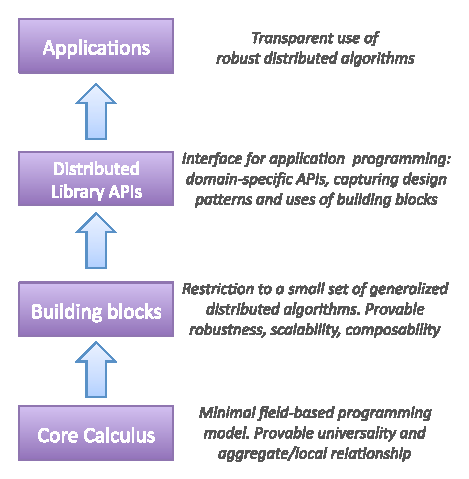
\includegraphics[width=0.6\textwidth]{res/fig/stack-2.eps}%
  \caption[
    Principali livelli dell'\emph{Aggregate Programming}.
  ]{
    Principali livelli dell'\emph{Aggregate Programming}.

    \nameCref{fig:stack} ripresa da~\cite{ProtelisSAC14}.
  }%
  \label{fig:stack}
\end{figure}

Nelle \nameCrefs{sec:field-calculus} successive analizzeremo più nel dettaglio alcuni di questi.

\section[Field calculus]{Field calculus \& Building Blocks}\label{sec:field-calculus}

Al livello più basso della struttura rappresentata in \Cref{fig:stack} si trova il \emph{field calculus}~\cite{FieldCalculusFOCLASA2013}.
Esso è un \emph{core calculus}, ovvero un modello teorico di programmazione che riassume la semantica operazionale minimale necessaria alla progettazione di un sistema aggregato.

Il field calculus si basato sul concetto di \emph{campo computazionale}~\cite{FieldCalculusFOCLASA2013}:
il termine riprende la nozione di campo in fisica~\cite{mcmullin2002origins}, esteso al concetto di computazione
e inteso come ``una proiezione di ciascun dispositivo computazionale nello spazio verso un oggetto computazionale arbitrario'',
ossia l'applicazione di una funzione che, in un dato momento nel tempo, mappa ogni punto dello spazio (un dispositivo o un nodo),
verso un oggetto computazionale (un valore) che rappresenta il risultato della computazione su quel device.
I \emph{campi} sono strutture dati distribuite a livello di aggregazione che gradualmente si adattano ai cambiamenti della topologia sottostante e alle interazioni con l'ambiente.

I campi vengono generati e manipolati attraverso cinque costrutti fondamentali~\cite{BV-FOCAS2014,computationalfields-forte2015}:

\unsure[inline]{
  Qui ho espresso gli operatori con la sintassi (mi pare di capire LISP-like, credo ripresa da Proto) che veniva utilizzata nei primi paper sull'argomento.

  Va bene? Oppure dovrei usare le notazioni che avete usato nei paper più recenti (che invece penso si appoggino alla sintassi Protelis)?
}

\begin{description}
  % TODO: should I use new notation?
  \item[Built-in operator] \((\,\texttt{b\,(e\textsubscript{1}\:\dots{}\:e\textsubscript{n})}\,)\) \\
    Un operatore \emph{built-in} \texttt{b} modella in modo uniforme operazioni basate su valori puntuali, cioè che non coinvolgono né lo stato, né la comunicazione.
    Esso determina il valore del campo in output all'evento \texttt{m} (un punto nello spazio-tempo) solo dai valori dello spazio \texttt{e}
    e dei campi in input \(\texttt{e\textsubscript{1}\:\dots{}\:e\textsubscript{n}}\).
    Possono essere funzioni \emph{stateless} matematiche, logiche o algoritmiche, ma anche sensori, attuatori, funzioni di libreria, ecc.
  % TODO: should I use new notation?
  \item[Function definition and call] \((\,\texttt{def\ f\,(x\textsubscript{1}\:\dots{}\:x\textsubscript{n})\ e}\,)\) \\
    Astrazione e ricorsione sono supportate attraverso la definizione di funzione:
    una funzione \texttt{f} con parametri formali \(\texttt{x\textsubscript{1}\:\dots{}\:x\textsubscript{n}}\) e corpo \texttt{e}
    può essere dichiarata con la sintassi \emph{Lisp-like} di cui sopra e invocata con \((\,\texttt{f\,(e\textsubscript{1}\:\dots{}\:e\textsubscript{n})}\,)\).
  % TODO: should I use new notation?
  \item[Time evolution] \((\,\texttt{rep\ x\;e\textsubscript{0}\;e}\,)\) \\
    Il costrutto di ripetizione supporta l'evoluzione dinamica dei campi, assumendo che ciascun dispositivo computi il proprio programma ripetutamente in \emph{round} asincroni.
    La variabile di stato \texttt{x} è inizializzata con il risultato della valutazione dell'espressione \texttt{e\textsubscript{0}} e aggiornato ad ogni step computando \texttt{e} in relazione al precedente valore di \texttt{x}.
  % TODO: should I use new notation?
  \item[Neighborhood values] \((\,\texttt{nbr\ e}\,)\) \\
    L'interazione diretta tra i dispositivi è incapsulata nel costrutto \texttt{nbr};
    con esso, si ottiene campo per ogni dispositivo, il quale è una mappa da tutti i vicini al loro più recente valore di \texttt{s}.
    Funzioni ``\emph{hood}'' \emph{built-in} possono poi riassumere queste mappe.
  % TODO: should I use new notation?
  \item[Domain restriction] \((\,\texttt{if\ e\textsubscript{0}\;e\textsubscript{1}\;e\textsubscript{2}}\,)\) \\
    La ramificazione distribuita è implementata dal costrutto \texttt{if}, che permette di suddividere la rete in due regioni:
    una nella quale l'espressione \texttt{e\textsubscript{0}} è vera, nel quale \texttt{e\textsubscript{1}} viene computato, e una nella quale è falsa, che invece computerà \texttt{e\textsubscript{2}}.
    Tali suddivisioni sono incapsulate e non possono avere effetti al di fuori dei relativi sottospazi.
\end{description}

Questi costrutti permettono al \emph{field calculus} di essere universale~\cite{beal2014towards}, supportando ogni computazione spazio-temporale causale e approssimabile.
Tramite questi operatori, inoltre, sono garantite:
\begin{inparaitem}
  \item \emph{portabilità},
  \item \emph{indipendenza} dall'infrastruttura,
  \item \emph{integrazione} con servizi non aggregati.
\end{inparaitem}

\unsure[inline]{
  Gli elenchi in-line a me piacciono per elenchi di singole parole, al posto di una semplice riga separata da virgole.

  So che da molti sono considerati accettabili solo per i paper con limite di lunghezza per risparmiare spazio in elenchi veri e propri, non per questo uso.
  Lei che ne pensa?
}

Per poter garantire anche \emph{resilienza} alla coordinazione, è necessario introdurre il livello di astrazione successivo:
gli operatori ``\emph{building block}''~\cite{BV-FOCAS2014}.

Questo layer consiste di un insieme di operatori generici e di più alto livello, che offrono allo sviluppatore un ambiente di programmazione più espressivo,
contribuendo in particolare alla cosiddetta \emph{self-stabilization}, ossia la capacità di raggiungere uno stato atteso in un numero finito di passi,
indipendentemente dallo stato di partenza.
Tale proprietà è garantita per tutti i campi ottenuti tramite composizione funzionale~\cite{BV-FOCAS2014}.

\begin{figure}[htbp]
  \centering
  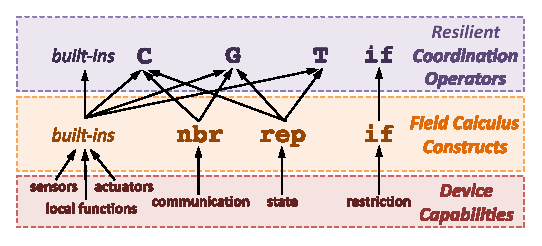
\includegraphics[width=0.8\textwidth]{res/fig/stack-detail-crop.eps}%
  \caption{Dettaglio dei livelli più bassi dell'\emph{Aggregate Programming}.}%
  \label{fig:stack-detail}
\end{figure}

Come riportato in~\Cref{fig:stack-detail}, i \emph{building block} individuati in aggiunta al costrutto \texttt{if} del \emph{field calculus} sono tre operatori di coordinazione~\cite{7274429,BV-FOCAS2014}:

\unsure[inline]{Qui mi rendo conto che le traduzioni sono brutte e verbose. Posso metterle in inglese?}

\unsure[inline]{Dovrei espandere la descrizione? Dovrei riportare il costrutto comprensivo di parametri? (con l'italiano non ci sta nella riga)}

\begin{description}
  \item[Diffusione dell'informazione nello spazio] \texttt{G} \\ % Spreading Information Across Space
    % \texttt{G(source, init, metric, accumulate)} \\ % ChkTeX 36
    Quest'operatore generalizza operazioni molto comuni come la stima della distanza e messaggi broadcast.
  \item[Raccoglimento di informazione attraverso lo spazio] \texttt{C} \\ % Collecting Information From Across Space
    % \texttt{C(potential, accumulate, local, null)} \\ % ChkTeX 36
    Quest'operatore aggrega le informazioni verso la sorgente attraverso il gradiente di un campo specificato.
  \item[Riassunto dell'informazione nel tempo] \texttt{T} \\ % Summarizing Information Across Time
    % \texttt{T(init, floor, decay)} \\ % ChkTeX 36
    Quest'operatore generalizza un timer il cui rateo di aggiornamento può variare nel tempo.
\end{description}

Questi operatori sono sufficientemente espressivi da poter coprire, da soli o combinati tra loro, tutti i pattern di coordinazione usati nei sistemi a larga scala.

Come livello di astrazione ulteriore (il secondo dall'alto nella~\Cref{fig:stack}), volto a semplificare la composizione dei \emph{building blocks}, si aggiungono le API \emph{general-purpose}~\cite{amslaurea13090}.
Esse possono essere usate e composte tra loro per scrivere applicazioni distribuite senza preoccuparsi dei meccanismi di coordinazione, la cui robustezza è garantita dagli operatori descritti sopra.

% \section[Protelis]{Protelis, Programming Language for Aggregate Computing}\label{sec:protelis}
\section{Protelis}\label{sec:protelis}

% \begin{wrapfigure}{r}{0.2\textwidth}
%   \begin{center}
%     
\includegraphics[width=0.2\textwidth]{res/fig/protelis-logo.png}%
%     \caption{Logo}%
%     \label{fig:protelis}
%   \end{center}
% \end{wrapfigure}

% \begin{wrapfigure}{r}{0pt}
%   \centering
%   % \vspace{-52pt}
%   
\includegraphics[width=0.2\textwidth]{res/fig/protelis-logo.png}
%   % \vspace{50pt}
%   \caption{Logo}%
%   \label{fig:protelis}
% \end{wrapfigure}

Field calculus è solamente un impianto teorico.
Vista la necessità di un'architettura portabile in grado di gestire gli aspetti di comunicazione, esecuzione e interfacciamento con hardware e sistema operativo, è stato realizzato Protelis.

\emph{Protelis}~\cite{PianiniSASOTutorial2017} è un linguaggio di programmazione aggregato di paradigma funzionale fortemente influenzato da Proto~\cite{Beal2006}.
Il linguaggio incorpora le principali funzionalità di computazione spaziale di field calculus in una sintassi più simile ai linguaggi strutturati tradizionali come C o Java.

\begin{figure}[htbp]
  \centering
  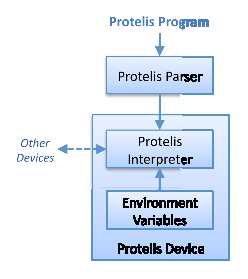
\includegraphics[width=0.4\textwidth]{res/fig/protelis-abstract-arch.eps}
  \caption[
    Architettura di Protelis
  ]{
    Architettura di Protelis.

    Figura ripresa da~\cite{ProtelisSAC14}.
  }%
  \label{fig:protelis-stack}
\end{figure}

% \begin{wrapfigure}{l}{0pt}
%   \centering
%   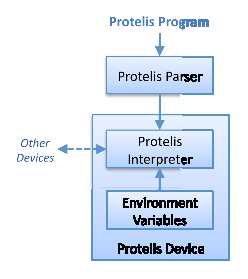
\includegraphics[width=0.4\textwidth]{res/fig/protelis-abstract-arch.eps}
%   \caption{Architettura di Protelis}%
%   \label{fig:protelis-stack}
% \end{wrapfigure}

Un nodo Protelis è costituito da un parser che traduce il programma in codice eseguibile, il quale è poi eseguito a intervalli regolari da un interprete, che si fa carico degli aspetti di interazione con il vicinato e con l'ambiente.
Ogni esecuzione è chiamata \emph{computational round}.

Il linguaggio e l'interprete sono basati su Java e possono essere inseriti in contesti virtuali~\cite{ProtelisSAC14} o reali indifferentemente.
Questo offre, da un lato, la portabilità e il supporto alle differenti piattaforme che la JVM (\emph{Java Virtual Machine}) mette a disposizione, dall'altro l'estendibilità che l'ecosistema di librerie Java può offrire.

Nel mondo scientifico, il linguaggio è già stato utilizzato per la realizzazione di diversi algoritmi aggregati.
Di seguito sono riportati alcuni esempi.

% \begin{itemize}
%   \item \emph{rendezvous} durante un evento di massa~\cite{ProtelisSAC14};
%   \item gestione di reti di servizi~\cite{7306601};
%   \item integrazione con servizi di realtà aumentata~\cite{PCRV-SCOPES2015}.
% \end{itemize}

\begin{description}
  % \item[Rendezvous durante un evento di massa]\cite{ProtelisSAC14}
  %   % Un problema tipico degli eventi di massa è la possibilità di due individui di incontrarsi in un determinato punto, in quanto la presenza elevata di dispositivi complica l'accesso a servizi cloud.
  %   Tramite Protelis, è stato possibile definire un algoritmo che consente a due persone che partecipano ad un evento di massa di incontrarsi in un punto intermedio, evitando le zone ad alta densità.

  % \item[Stima di pericolosità di una zona]\cite{BV-FOCAS2014}
  %   Basandosi sulla densità dei dispositivi in una zona, è stato possibile stimarne la pericolosità e definire modalità di dispersione efficaci.

  % \item[Algoritmi legati all'affollamento]
  %   Un problema tipico degli eventi di massa è la possibilità di due individui di incontrarsi in un determinato punto.
  %   Tramite Protelis, è stato possibile definire un algoritmo di \emph{rendezvous}~\cite{ProtelisSAC14} in grado di evitare le zone ad alta densità.

  %   In un altro progetto, basandosi sulla densità dei dispositivi in una zona, è stato possibile stimarne la pericolosità e definire modalità di dispersione efficaci.

  \item[Algoritmi legati all'affollamento]
    Tramite Protelis, è stato possibile~\cite{BV-FOCAS2014} stimarne la pericolosità di una data zona nell'ambiente basandosi sulla densità dei dispositivi presenti e definire modalità di dispersione efficaci.

    In un altro progetto~\cite{ProtelisSAC14}, è stata definito un algoritmo di \emph{rendezvous} in grado di evitare le zone ad alta densità nel contesto di un evento di massa, permettendo l'incontro di due individui in un punto intermedio.

  \item[Gestione di reti di servizi]\cite{7306601}
    Un altro utilizzo significativo è stato per la realizzazione di un sistema di gestione tra servizi in rete.
    Tali servizi, talvolta datati, possono avere molte dipendenze tra loro e scarse capacità di coordinazione.
    Per evitare stati di inconsistenza, spesso l'ordine di arresto dei server è strettamente legato alle dipendenze e rende difficile l'automazione.

    Utilizzando Protelis è stato possibile realizzare un sistema in grado di organizzarsi per riavviare lo stack.
    In particolare, sono state definite entità chiamate \emph{daemon} che monitorano ciascuna uno specifico servizio e comunicano con le altre al fine di garantire l'ordine necessario.

  \item[Integrazione con servizi di realtà aumentata]\cite{PCRV-SCOPES2015}
    La programmazione aggregata è stata testata anche nell'ambito dell'AR (\emph{Augmented Reality}).

    % In particolare, è stato introdotto il concetto di \emph{campo aumentato} che combina i campi computazionali con le capacità dell'AR\@.
    Ad esempio, è possibile utilizzare visori di realtà aumentata per visualizzare nell'ambiente i campi computazionali
    o, viceversa, modellare i dati raccolti da sensori AR come campi (detti \emph{augmented fields}).
\end{description}

\unsure[inline]{Dovrei aggiungere altri dettagli su Protelis?}

% \section[ScaFi]{ScaFi, Aggregate Programming Toolkit}\label{sec:scafi}
\section{ScaFi}\label{sec:scafi}

Una tecnologia analoga è rappresentata da \emph{ScaFi} (\emph{\emph{Sca}la with computational \emph{Fi}elds})~\cite{aggregatescala-pmldc2016}:
si tratta di un framework in Scala per la realizzazione di programmi aggregati attraverso un set compatto di primitive, presentato come implementazione del field calculus alternativa a Protelis.
% Nonostante sia dunque un DSL di Scala, è sufficientemente completo da poter essere considerato un linguaggio di programmazione aggregata a sé stante.

Il framework è composto principalmente da due parti:

% \begin{itemize}
%   \item una piattaforma distribuita che permette la configurazione e l'esecuzione di sistemi aggregati.
%   \item un \emph{internal DSL} (\emph{Domain Specific Language}) di Scala che fornisce la sintassi e la semantica per i costrutti base del field calculus.
% \end{itemize}

\begin{description}
  \item[Aggregate programming support]
    La seconda parte è un \emph{internal DSL} (\emph{Domain Specific Language}) di Scala che fornisce la sintassi e la semantica per i costrutti base del field calculus.

  \item[Aggregate platform support]
    La prima parte è una piattaforma distribuita basata sul modello ad attori di Akka che permette la configurazione e l'esecuzione di sistemi aggregati.
    Essa può essere utilizzata in modalità decentralizzata (\emph{peer-to-peer} %, \Cref{fig:scafi:p2p}
    ) o in modalità centralizzata (\emph{server-based}%, \Cref{fig:scafi:server-based}                  % ChkTeX 37
    ).                                                                                                  % ChkTeX 37

    % \begin{figure}[htbp]
    %   \centering
    %   \begin{subfigure}{0.35\textwidth}
    %     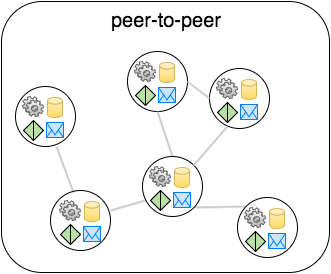
\includegraphics[width=\textwidth]{res/fig/scafi-p2p.png}
    %     \caption{Architettura \emph{peer-to-peer}}%
    %     \label{fig:scafi:p2p}
    %   \end{subfigure}
    %   \hspace{0.15\textwidth} % a differenza di \hfill il commento serve per non aggiungere spazi
    %   \begin{subfigure}{0.35\textwidth}
    %     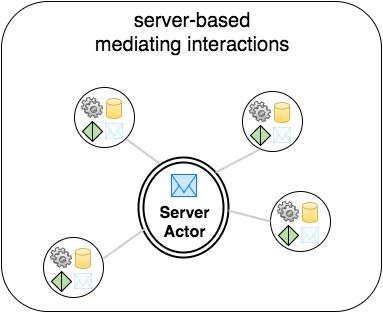
\includegraphics[width=\textwidth]{res/fig/scafi-server-based.png}
    %     \caption{Architettura \emph{server-based}}%
    %     \label{fig:scafi:server-based}
    %   \end{subfigure}
    %   \caption[
    %     Architetture della piattaforma distribuita di ScaFi
    %   ]{
    %     Architetture della piattaforma distribuita di ScaFi.

    %     Figura ripresa da~\cite{AggregatecomputingVlsubicomp16}.
    %   }%
    %   \label{fig:scafi}
    % \end{figure}

    Nel caso centralizzato, la piattaforma mantiene le posizione spaziali dei dispositivi e gestisce il vicinato, secondo il modello tradizionale client-server.
\end{description}

Basandosi su Scala come linguaggio ospite, è in grado di interoperare con Java e gli altri linguaggi in grado si eseguire in ambiente JVM, mantenendo il solido \emph{type-system} messo a disposizione da Scala e i suoi costrutti funzionali.

\unsure[inline]{Dovrei aggiungere altri dettagli su Scafi?}
